The final application of the feature detection and matching algorithms is the computation of a visual odometry.
Only the promising candidates \acrshort{sift} and \acrshort{akaze} are compared.
Both feature images and the color images are used separatly to determine the visual odometry for a given trajectory, the groundtruth.

\acrshort{sift} neither results in a good odometry for color images nor for the feature images.
Figure~\ref{fig:sift_odometry} shows random turns and barely straight trajectories for any conversion.
\begin{figure}[t]
\begin{subfigure}[b]{0.31\linewidth}
    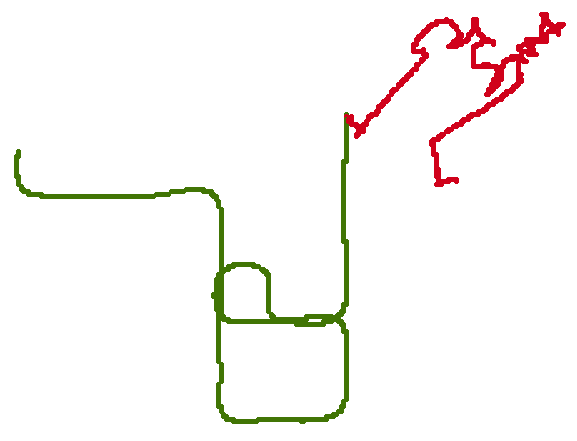
\includegraphics[width=\linewidth]{chapter06/odo/jonas_flexion_SIFT_nice.png}%
    \caption{\glspl{flexion-image}}
\end{subfigure}%
\begin{subfigure}[b]{0.31\linewidth}
    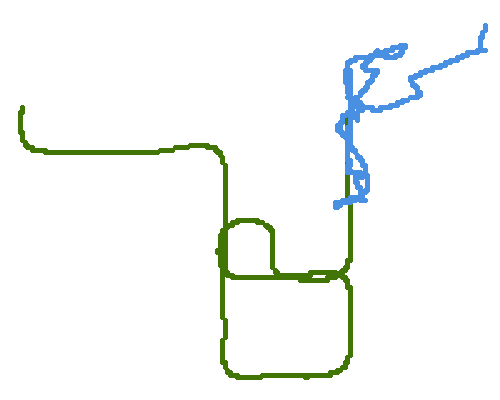
\includegraphics[width=\linewidth]{chapter06/odo/jonas_bearing_SIFT_nice.png}%
    \caption{\glspl{bearing-angle-image}}
\end{subfigure}%
\begin{subfigure}[b]{0.31\linewidth}
    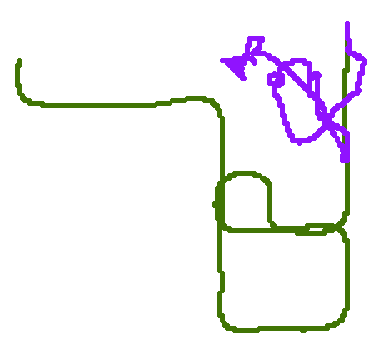
\includegraphics[width=0.8\linewidth]{chapter06/odo/zhang_pinhole_SIFT_nice.png}%
    \caption{Color Images}
\end{subfigure}
\caption[\acrshort{sift} odometry trajectories compared]{\emph{\acrshort{sift} odometry trajectories compared.} The presented odometry trajectories for the benchmark dataset from Zhang et al.\cite{zhang_icra2016} are calculated with an in-house implementation of a basic visual odometry system using \acrshort{sift}.}\label{fig:sift_odometry}
\end{figure}
\acrshort{akaze} on the other hand performs much better in all cases, as can be seen in Figure~\ref{fig:akaze_odometry}.
The prinicpal shape of the trajectory is reconstructed well.
The \glspl{bearing-angle-image} have higher drift compared to the \glspl{flexion-image} or colored images, but only in certain areas where all inputs suffer from similar issues.
\begin{figure}[b!]
\begin{subfigure}[t]{0.31\linewidth}
    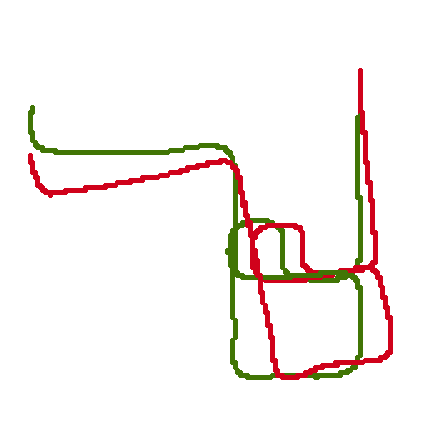
\includegraphics[width=\linewidth]{chapter06/odo/jonas_flexion_AKAZE_nice.png}%
    \caption{\glspl{flexion-image}}
\end{subfigure}%
\begin{subfigure}[t]{0.31\linewidth}
    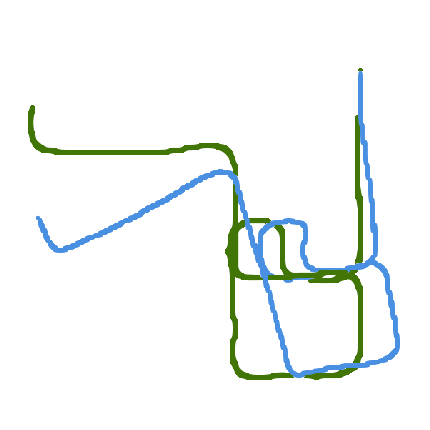
\includegraphics[width=\linewidth]{chapter06/odo/jonas_bearing_AKAZE_nice.png}%
    \caption{\glspl{bearing-angle-image}}
\end{subfigure}%
\begin{subfigure}[t]{0.31\linewidth}
    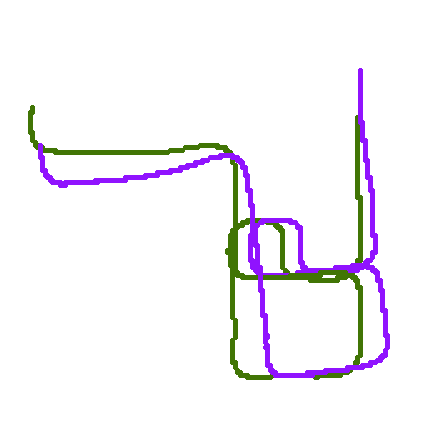
\includegraphics[width=\linewidth]{chapter06/odo/zhang_pinhole_AKAZE_nice.png}%
    \caption{Color Images}
\end{subfigure}
\caption[\acrshort{akaze} odometry trajectories compared]{\emph{\acrshort{akaze} odometry trajectories compared.} The presented odometry trajectories for the benchmark dataset from Zhang et al.\cite{zhang_icra2016} are calculated with an in-house implementation of a basic visual odometry system using \acrshort{akaze}.}\label{fig:akaze_odometry}
\end{figure}
The findings show that the higher number of keypoints results in better localization performance.
Because the benchmark dataset is a synthetic, the colored image do not contain the same level of texture as in real life.
This explains the bad performance of \acrshort{sift} for the colored images.
The range data conversions on the other hand are representative for real world cases.
A higher number of keypoints, combined with false positive rejection through \acrshort{RANSAC} are enough to yield odometry performance similar to colored images.
